\documentclass[11pt]{article}
\usepackage{amsmath,amsthm,amssymb,fullpage,graphicx,hyperref,listings}
\usepackage{listings,color,setspace}
\author{Andy Reagan}
\title{Math 337 Homework 04}

     \def\NN{\mathbb{N} }
     \def\ZZ{\mathbb{Z} }
     \def\QQ{\mathbb{Q} }
     \def\RR{\mathbb{R} }
     \def\CC{\mathbb{C} }
     \def\f{\frac }
     \def\b{\begin }
     \def\e{\end }
     \def\Log{\text{Log} \,}
     \def\Re{\text{Re} \, }

\lstset{language=MATLAB,
basicstyle=\ttfamily\scriptsize\singlespacing,
keywordstyle=\color{blue},
stringstyle=\color{red},
commentstyle=\color{green},
morecomment=[l][\color{magenta}]{\#},
frame=L,
xleftmargin=\parindent,
%%numbers=left,                   %% where to put the line-numbers
%%numberstyle=\scriptsize,      %% the size of the fonts that are used for the line-numbers
%%stepnumber=1,                   %% the step between two line-numbers. If it is 1 each line will be numbered
numbersep=5pt,
breaklines=true,        %% sets automatic line breaking
breakatwhitespace=false,    %% sets if automatic breaks should only happen at whitespace
escapeinside={\%*}{*)} 
}

\begin{document}
\maketitle

\begin{enumerate}

\item For the Modified Euler method, obtain Equations 4.21 and 4.22.
Then plot the stability region boundary given by 4.22.

\bigskip
\textbf{Solution:} Writing out the ME method as a difference equation, we have:
\begin{equation} Y_{i+1} = Y_i + \f{1}{2} h f(x_i,Y_i) + \f{1}{2} hf(x_i+h,Y_i + hf(x_i, Y_i)) .\end{equation}
Plugging in the model problem, $f(x,y) = \lambda y$, we have the difference equation
\begin{align} Y_{i+1} &= Y_i + \f{1}{2}h  \lambda Y_i + \f{1}{2} h \lambda Y_i + \f{1}{2} h \lambda h f(x_i, Y_i))\\
&= Y_i + h  \lambda Y_i + \f{1}{2} \lambda h^2 \lambda Y_i \\
&= Y_i + h  \lambda Y_i + \f{1}{2} (h\lambda)^2 Y_i \\
&= Y_i \left( 1 + h  \lambda + \f{1}{2} (h\lambda)^2 \right ) .\end{align}
The above Equation 5 is the desired form of Equation 4.21 from the notes.
Since this equation approximates the growth rate of the error, for the method to be stable we require the RHS be less than one in magnitude (modulus), and for complex $\lambda$ we write the boundary of this region this as
\begin{equation} \left | 1 + h  \lambda + \f{1}{2} (h\lambda)^2 \right | = 1 .\end{equation}
Writting $\lambda = \lambda _R + i \lambda _I$ we have, equivalently,
\begin{equation} \left ( 1 + h  \lambda_R + \f{1}{2} (h\lambda_R)^2 - \f{1}{2} (h\lambda_I)^2 \right ) + \left ( h  \lambda_I + h^2\lambda_I\lambda_R \right ) ^2= 1 .\end{equation}

The following code makes a plot:
\lstinputlisting[language=Matlab]{andy_hw04_prb01.m}

\begin{figure}[h!]
  \centering
    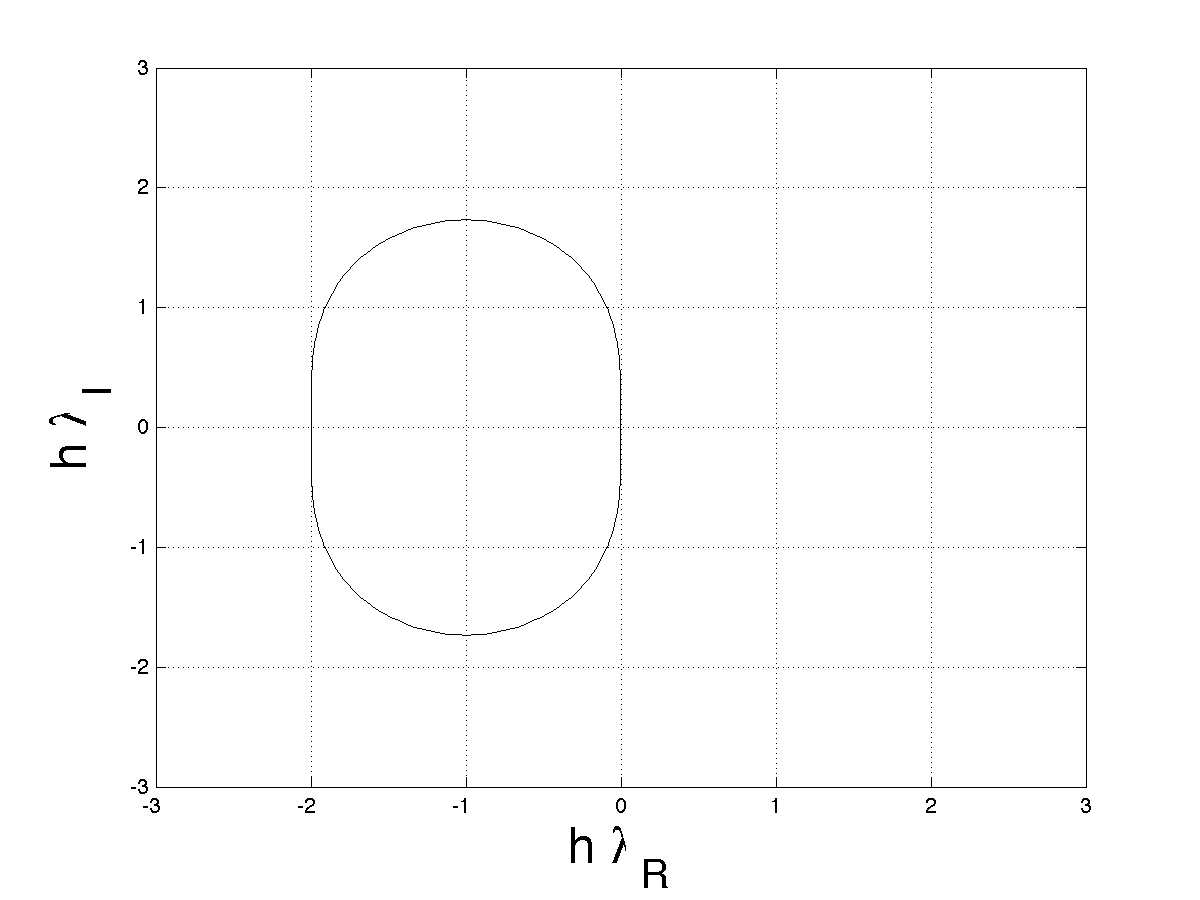
\includegraphics[width=0.8\textwidth]{andy_hw04_prb01.png}
  \caption{Stability of the ME method.}
\end{figure}

\pagebreak
\item Use inequality 4.23 to obtain the bound 4.24 for the stability of the cRK method when $\lambda < 0$.

\bigskip
\textbf{Solution:} From Equation 4.23, the cRK method is stable when
\begin{equation} \left | \sum _{k=0} ^4 \f{(h\lambda) ^k}{k!} \right | \leq 1 .\end{equation}
Taking the simple route, we make a plot of this function, and note where it becomes greater than one:

\lstinputlisting[language=Matlab]{andy_hw04_prb02_a.m}

Increasing the number of points in the above plot, this code then tells us that the stable region is $-2.784878 \leq h\lambda \leq 0.000$.

\begin{figure}[h!]
  \centering
    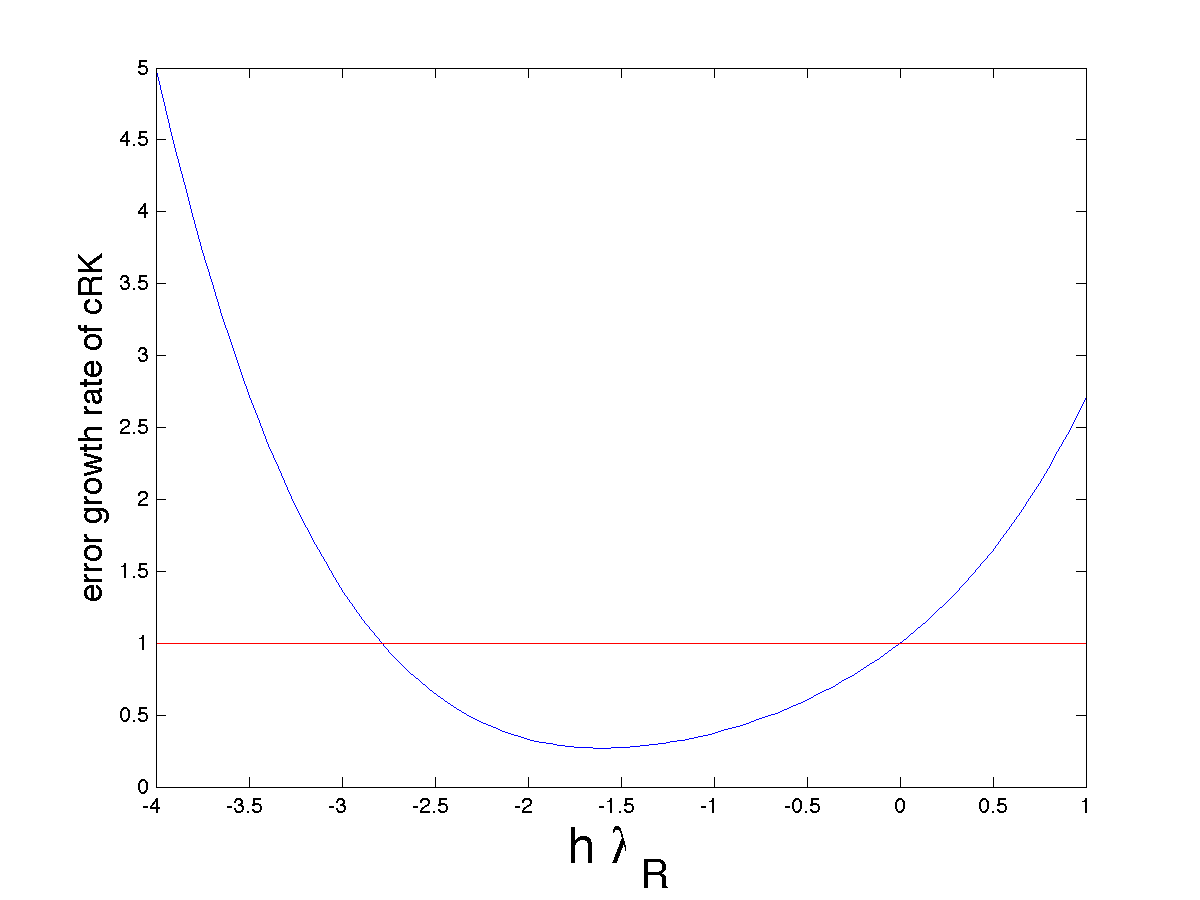
\includegraphics[width=0.5\textwidth]{andy_hw04_prb02_01.png}
  \caption{Stability of the cRK method.}
\end{figure}

\clearpage
\newpage
\item Show analytically that the stability region of the Midpoint method coincides with that for the ME method.

\textbf{Solution:} Similar to problem 1, we begin by writing the midpoint method in one step:
\begin{equation} Y_{i+1} = Y_i + hf(x_i+h/2,Y_i + h/2\cdot f(x_i, Y_i)) .\end{equation}
Plugging in the model problem, $f(x,y) = \lambda y$, we have the difference equation
\begin{align} Y_{i+1} &= Y_i + h \lambda Y_i + \f{1}{2} h \lambda h f(x_i, Y_i))\\
&= Y_i + h  \lambda Y_i + \f{1}{2} \lambda^2 h^2 Y_i \\
&= Y_i \left( 1 + h  \lambda + \f{1}{2} (h\lambda)^2 \right ) \label{prb3eq1}.\end{align}
This equation is the same as Equation 5, but we could continue and we have the stability region as, again,
\begin{equation} \left | 1 + h  \lambda + \f{1}{2} (h\lambda)^2 \right | = 1 ,\end{equation}
as desired.

\clearpage
\newpage
\item Use Equations 4.27 and 4.30 to plot the boundary of the stability region of the 2nd-order Adams-Bashforth method.

\textbf{Solution:} From the notes, we have the boundary of the stability region given by both $| r_1 | \leq 1$ and $| r_2 | \leq 1$ for $r_1,r_2$:
\begin{align} r_1 &= \f{1}{2} \left \{ \left ( 1+ \frac{3}{2} \lambda h \right ) \sqrt{\left ( 1 + \f{3}{2} \lambda h \right ) ^2 - 2\lambda h } \right \} . \end{align}

\lstinputlisting[language=Matlab]{andy_hw04_prb04.m}

\begin{figure}[h!]
  \centering
    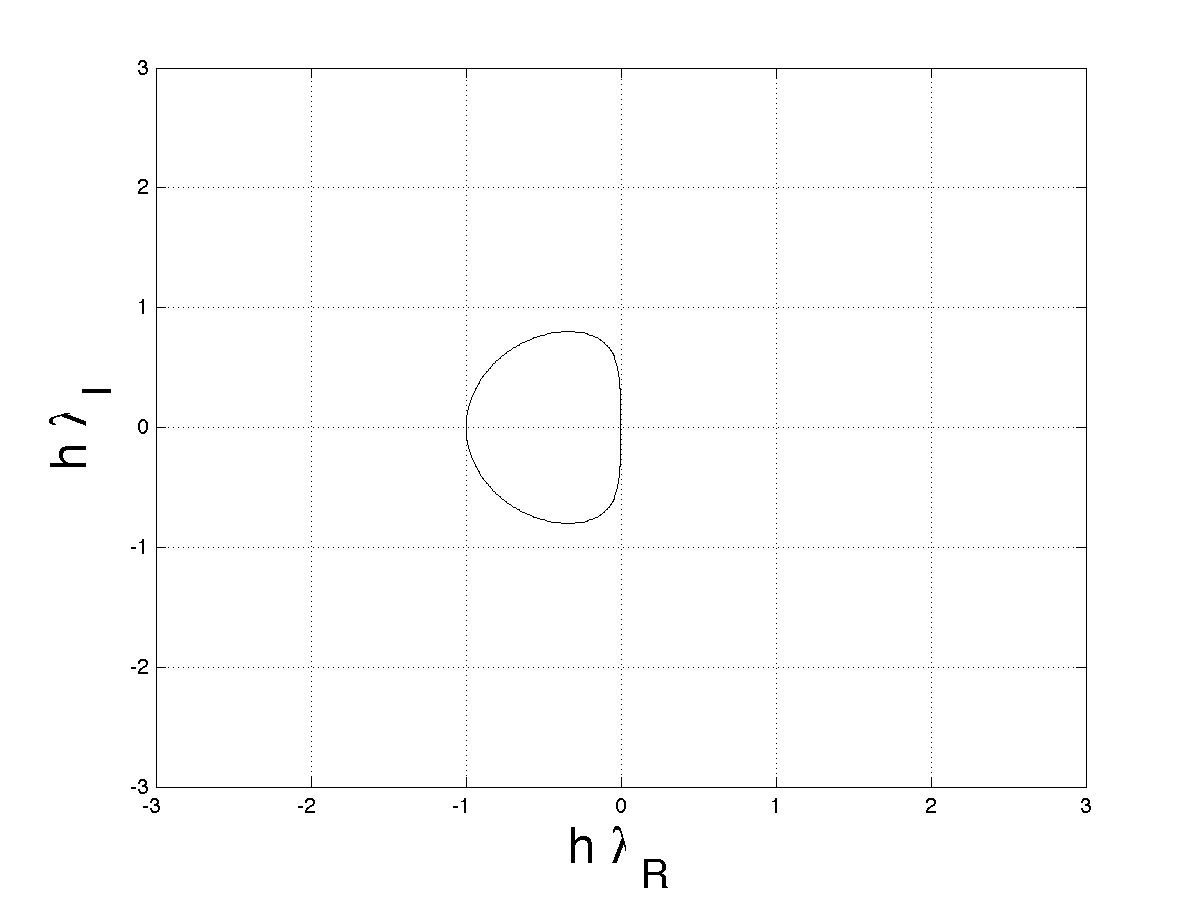
\includegraphics[width=0.8\textwidth]{andy_hw04_prb04_02.png}
  \caption{Stability of the 2nd-order Adams Bashforth method.}
\end{figure}

%% \begin{figure}[h!]
%%   \centering
%%     \includegraphics[width=0.8\textwidth]{}
%%   \caption{}
%% \end{figure}

\clearpage
\newpage
\item Obtain the analog of Equations 4.26 and 4.27 for the P-C method (3.33) of Lecture 3.
Plot its stability region following the suggestions of Problem 4.
Is this stability region larger or smaller than that of the 2nd-order Adams-Bashforth method?
In general, try to make an educated guess about how the stability region of a P-C method is related to the stability regions of its predictor and corrector equations.

\textbf{Solution:} The P-C method is given by equation 3.33 from Lecture 3, which is:
\begin{align} \text{Predictor}~:~~ Y_{i+1} ^p & = Y_i + h/2 \cdot ( 3f_i - f_{i-1} ) \\
\text{Corrector}~:~~ Y_{i+1} ^c & = Y_i + h/2 \cdot ( f_i + f^p_{i+1} ) .\end{align}
Writing this as one equation, we have
\begin{align} Y_{i+1} &= Y_i + h/2 \cdot \left( \lambda Y_i + \lambda \left ( Y_i + h/2 \cdot (3 \lambda Y_i - \lambda Y_{i-1}) \right ) \right ) \\
 &= Y_i + \f{1}{2} \lambda h Y_i + \frac{1}{2} \lambda h Y_i + \frac{3}{4} \lambda ^2 h^2 Y_i - \frac{1}{4} \lambda ^2 h^2 Y_{i-1} \\
 &= Y_i + \lambda h Y_i + \frac{3}{4} \lambda ^2 h^2 Y_i - \frac{1}{4} \lambda ^2 h^2 Y_{i-1} \end{align}

I switch now from subscripts $Y_i$ to $Y_n$ for less confusion with the imaginary unit.
Writing this as a difference equation we have
\begin{align} & Y_{n+1} - Y_n - \lambda h Y_n - \frac{3}{4} \lambda ^2 h^2 Y_n + \frac{1}{4} \lambda ^2 h^2 Y_{n-1}  = 0.\end{align}
Substituting $Y_n = r^n$ in the above, we have
\begin{align} r^{n+1} - r^n - \lambda h r^n - \frac{3}{4} \lambda ^2 h^2 r^n + \frac{1}{4} \lambda ^2 h^2 r^{n-1}   = 0.\end{align}
Cancelling the $r^{n-1}$ this becomes
\begin{align} r^2 + r \left ( -1 - \lambda h - \frac{3}{4} \lambda ^2 h^2 \right ) + \frac{1}{4} \lambda ^2 h^2 = 0.\end{align}

Solving this for the roots of $r$ we have the roots
\begin{align}  r_2 &= \frac{1}{2} \left \{ 1 + \lambda h + \frac{3}{4} \lambda ^2 h^2 + \sqrt{\left( 1 + \lambda h + \frac{3}{4} \lambda ^2 h^2 \right )^2 -\lambda^2 h^2 } \right \} \\
r_2 &= \frac{1}{2} \left \{ 1 + \lambda h + \frac{3}{4} \lambda ^2 h^2 - \sqrt{\left( 1 + \lambda h + \frac{3}{4} \lambda ^2 h^2 \right )^2 -\lambda^2 h^2 } \right \} \end{align}

The following code plots the boundary of the stable region.

The stability region is larger than that of the Adams-Bashforth method alone, indicating that the P-C scheme has improved the stability.

In general, I expect the stable region of a P-C method to be a constrained union of the stable regions of the predictor and corrector methods individually.
More specifically, I expect that the stable region behaves as the product of the stability (the error growth rate) of the two methods.
If this product is less than one, than the combined P-C method would be stable.
Otherwise, it will remain unstable.

\lstinputlisting[language=Matlab]{andy_hw04_prb05.m}

\begin{figure}[h!]
  \centering
    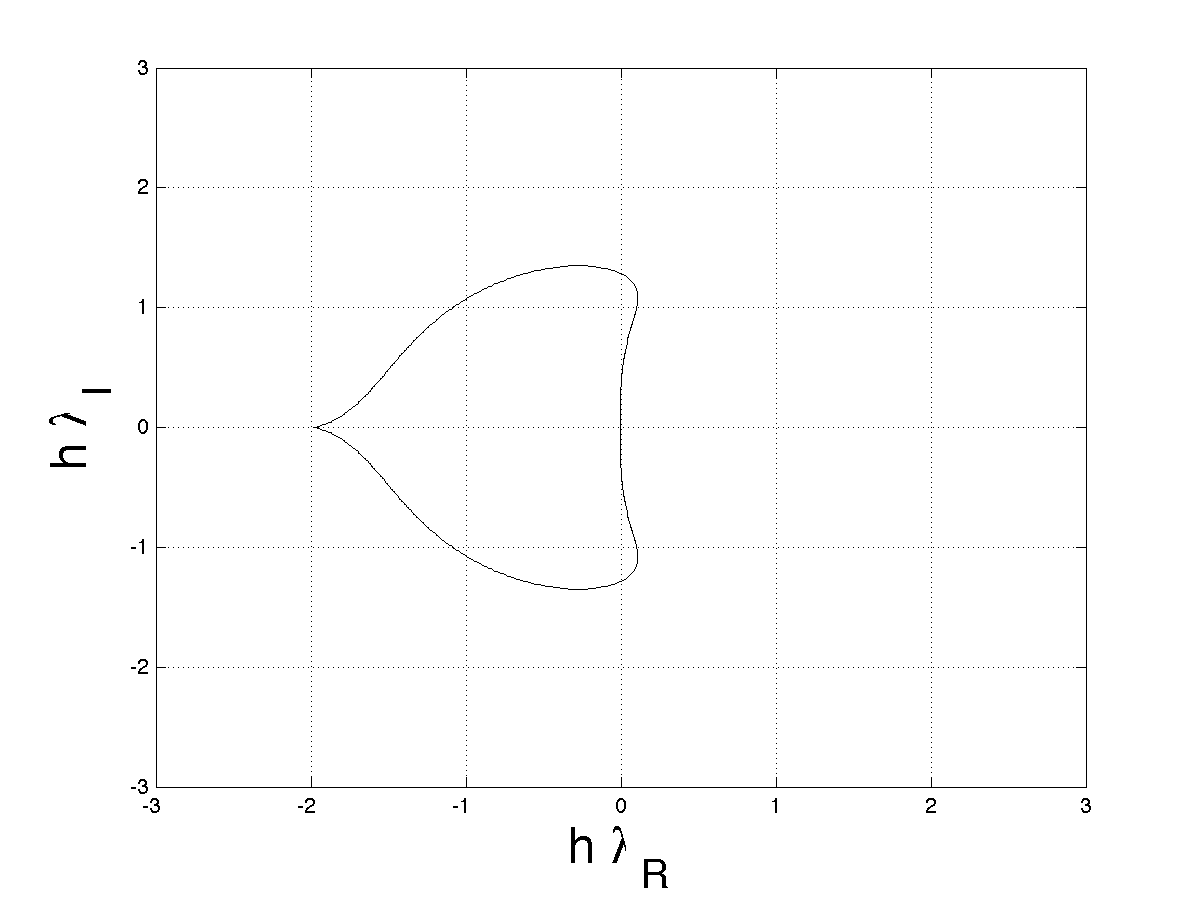
\includegraphics[width=0.8\textwidth]{andy_hw04_prb05_02.png}
  \caption{Stability of the P-C method given in Equation 3.33 from Lecture 3.}
\end{figure}

\clearpage
\newpage
\item Find {\em analytically} the stability region of the Modified Implicit Euler method (3.43) and make a sketch of the this region.
Explain why your result implies that this method is A-stable.

\textbf{Solution:} The modified Euler method is given by
\begin{equation} Y_{i+1} = Y_i + \f{h}{2} \left ( f(x_i,Y_i) + f(x_{i+1},Y_{i+1})\right ) . \end{equation}

Expanding this equation for the the model equation (4.15) we have
\begin{align} Y_{i+1} &= Y_i + \f{h}{2} \left ( \lambda Y_i + \lambda Y_{i+1}\right ) \\
&= Y_i (1+h\lambda /2) + h \lambda /2 \cdot Y_{i+1}. \end{align}
Rearranging this we have
\begin{align} Y_{i+1}(1-h\lambda /2) &= Y_i (1+h\lambda /2) . \end{align}
Recognizing this as a recursion, we write
\begin{align} Y_{n} &= Y_0 \left ( \frac{1+h\lambda /2 }{1-h\lambda /2} \right )^n . \end{align}
The modified Implicit Euler method is therefore stable for 
\begin{align} \left | \frac{1+h\lambda /2}{1-h\lambda /2} \right | \leq 1 ~~~~~~\Rightarrow ~~~~~~ \left | 1+h\lambda /2 \right |  \leq  \left | 1-h\lambda /2 \right |. \end{align}

This inequality clearly holds for all $\lambda < 0$, making the method A-stable.
I utilize the contour plotting scripts given above to make a plot of this region:
\lstinputlisting[language=Matlab]{andy_hw04_prb06.m}

Which makes the plot:
\begin{figure}[h!]
  \centering
    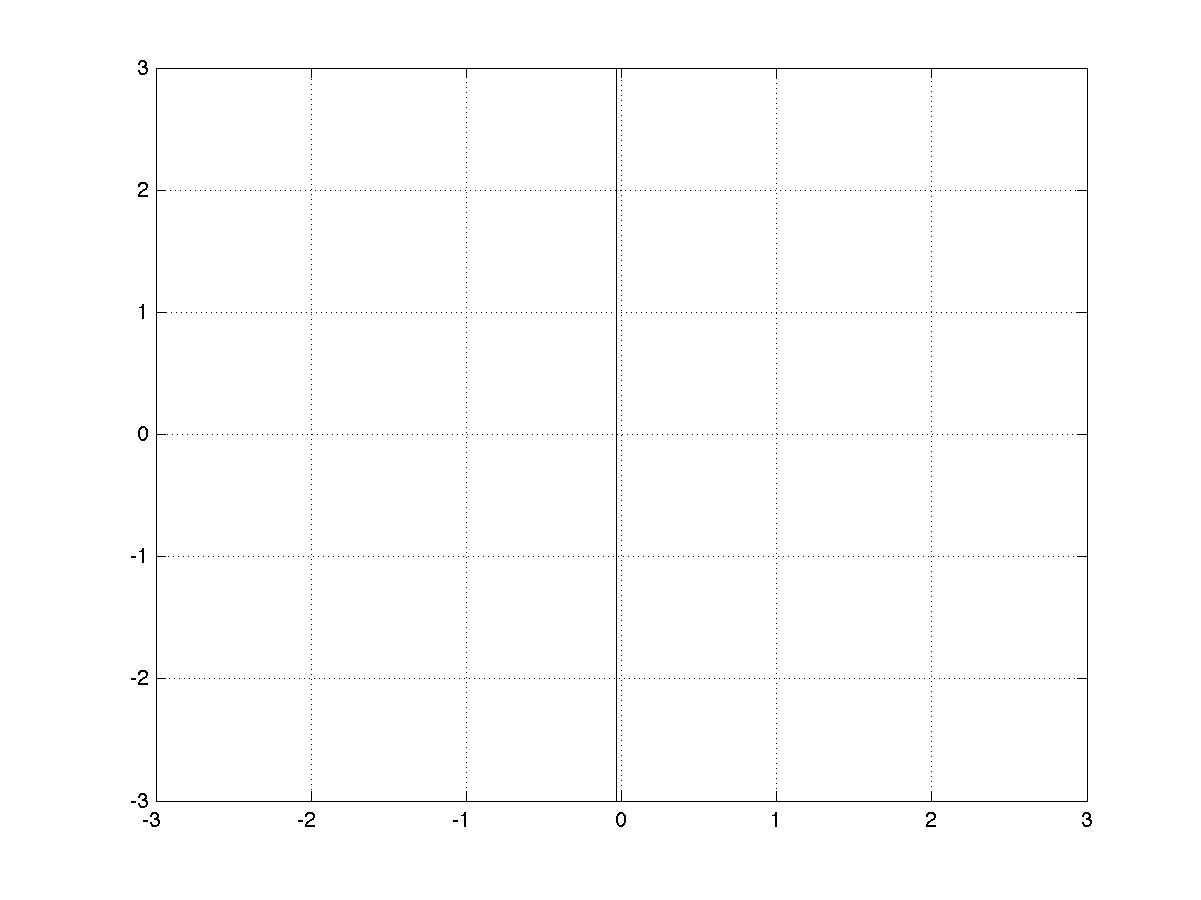
\includegraphics[width=0.8\textwidth]{andy_hw04_prb06_01.png}
  \caption{Stable region of the modified Euler method.}
\end{figure}

I also make a sketch of this region:
\begin{figure}[h!]
  \centering
    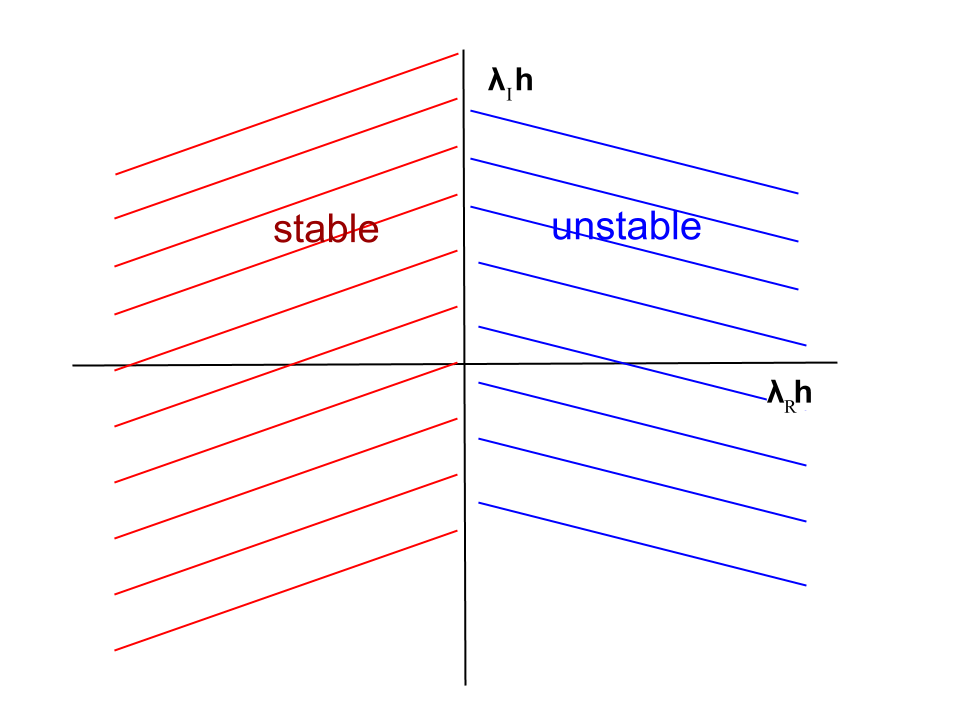
\includegraphics[width=0.8\textwidth]{andy_hw04_prb06_02.png}
  \caption{Sketch of the stable region of the modified Euler method.}
\end{figure}

\clearpage
\newpage
\item Solve the IVP 
\[ y' = 20y, ~~~~~~~~~~y(0)=1 \]
with $h=0.125$ up to $x=1.5$ using (a) simple Euler, (b) cRK, (c) implicit Euler methods.
Plot your result from (a).
In a separate figure, plot your results from (b) and (c) along with the exact solution.
Which method, the 4-th order (b), or the 1st-order (c), gives the more accurate solution in this case?

Without doing additional calculations, what do you expect to change in those results if you use $h=0.15$ instead?
Write a bried but coherent paragraph explaining your answer.

\textbf{Solution:} I solve the ODE using the given methods in the following MATLAB script:

\lstinputlisting[language=Matlab]{andy_hw04_prb07.m}

The plots are produced from this script directly. They are as follows.

\begin{figure}[h!]
  \centering
    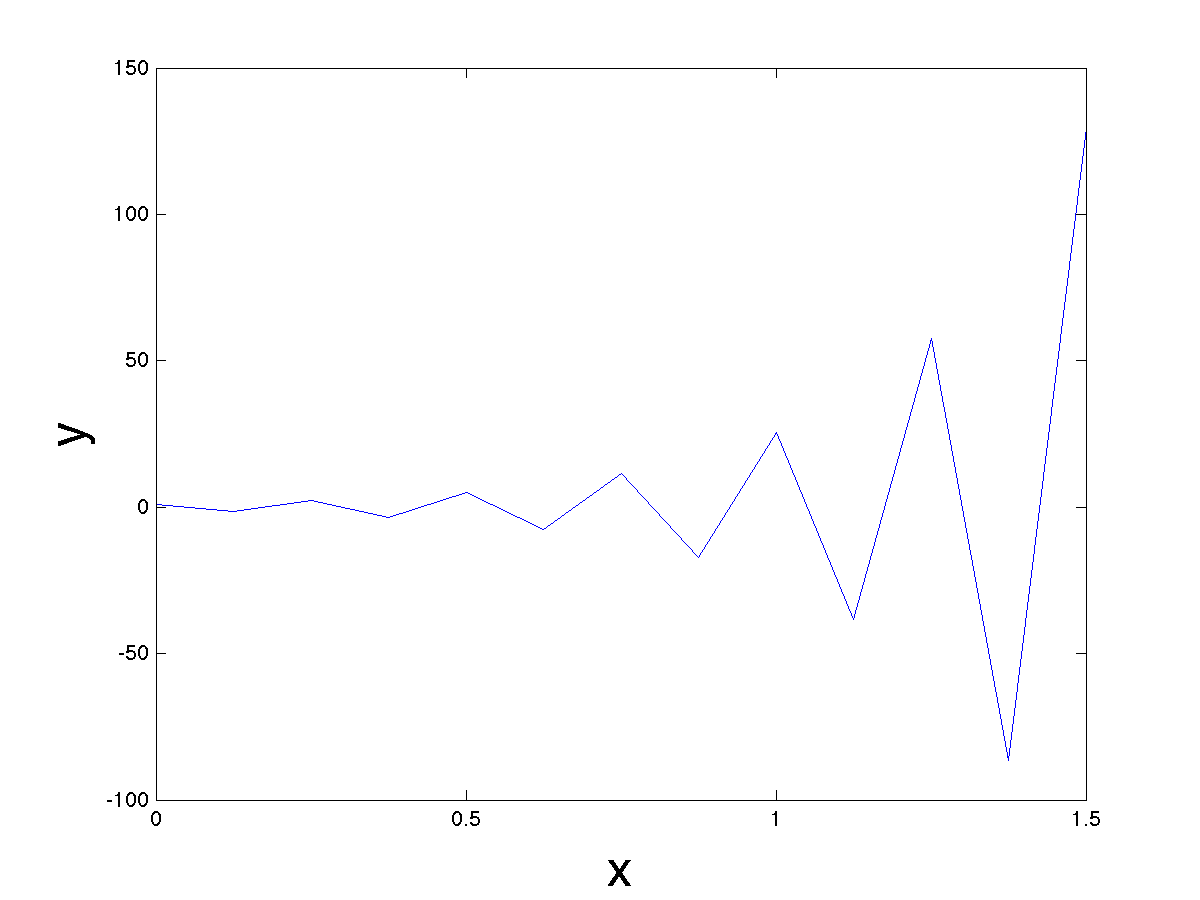
\includegraphics[width=0.8\textwidth]{andy_hw04_prb07_01.png}
  \caption{Solution with the simple Euler method.}
\end{figure}

\begin{figure}[h!]
  \centering
    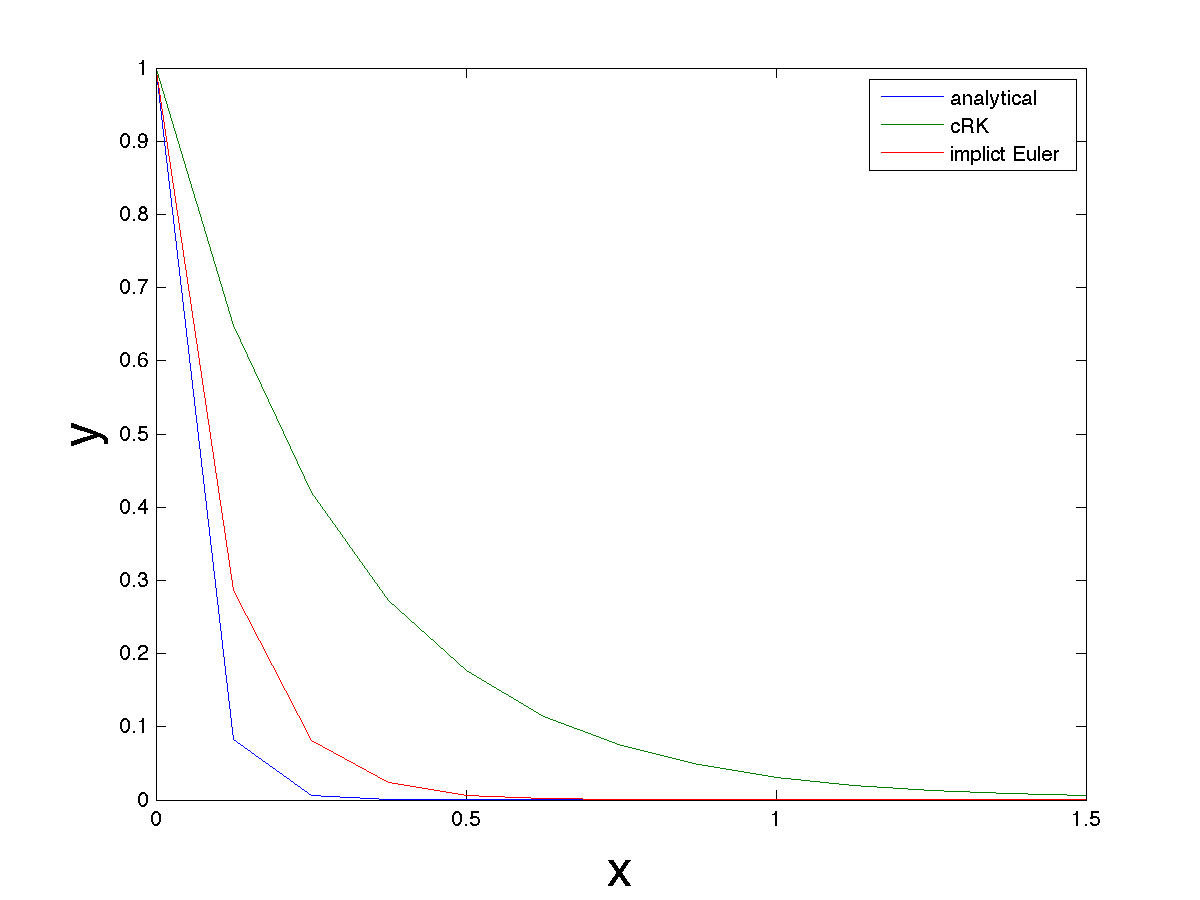
\includegraphics[width=0.8\textwidth]{andy_hw04_prb07_02.png}
  \caption{The exact, cRK, and implicit Euler solutions.}
\end{figure}

We observe that the 1st-order implicit Euler method is more accurate in this case.
An increase in $h$ will move $\lambda h$ further away from the stable region for the cRK method, yet remain within the stable region of the implicit Euler method.
For this reason, I would expect that the implicit Euler solution would improve while the cRK solution would become less stable, and likely degrade in accuracy.

\clearpage
\newpage
\item[Bonus] As shown in the notes, the Leap-frog method, introduced in Lecture 3, is unstable for $\lambda < 0$.
Now, construct a P-C method where the Leap-frog method is used as the predictor and the trapezoial rule is used as the corrector (as in method (3.33)).
Repeat Problem 5 for this new P-C method.

How does this region compare with the stability regions of the predictor equation and of the corrector equation alone?
Does this graph agree with what you observed in problem 5?

\textbf{Solution:} We write this P-C method as:
\begin{align} \text{Predictor}~:~~ Y_{i+1} ^p & = Y_{i-1} - 2hf(x_i,Y_i) \\
  \text{Corrector}~:~~ Y_{i+1} ^c & = Y_i + h/2 \cdot ( f(x_i,Y_i) + f(x_{i+1},Y^p_{i+1} ) .\end{align}
This problem now closely follows the Problem 5.
We write out this method in one step as:
\begin{align} Y_{i+1} & = Y_i + h/2 \cdot ( f(x_i,Y_i) + f(x_{i+1},Y_{i-1} - 2hf(x_i,Y_i) ) ).\end{align}
Substituting in the model equation we have:
\begin{align} Y_{i+1} & = Y_i + h/2 \cdot ( \lambda Y_i + \lambda Y_{i-1} - \lambda 2h \lambda Y_i ) \\
& = Y_i + h/2 \lambda Y_i + h/2 \lambda Y_{i-1} - h/2 \lambda 2h \lambda Y_i \\
& = Y_i (1 + h\lambda /2  - (h\lambda)^2 ) + Y_{i-1} (h\lambda /2) \end{align}

Substituting $Y_n = r^n$ in the above, we have
\begin{align} r^{n+1} - r^n (1 + h\lambda /2  - (h\lambda)^2 ) - r^{n-1} (h\lambda /2) = 0.\end{align}
Cancelling the $r^{n-1}$ this becomes
\begin{align} r^{2} - r (1 + (h\lambda) /2  - (h\lambda)^2 ) - (h\lambda) /2 = 0.\end{align}

Let $z$ denote $h\lambda$.
Solving the previous equation for the roots of $r$ we have the roots
\begin{align} r_1 &= \frac{1}{2} \left \{ 1 + (h\lambda) /2  - (h\lambda)^2 + \sqrt{\left( 1 + (h\lambda) /2  - (h\lambda)^2 \right ) ^2 + 2 \lambda h } \right \} \\
r_2 &= \frac{1}{2} \left \{ 1 + (h\lambda) /2  - (h\lambda)^2 - \sqrt{\left( 1 + (h\lambda) /2  - (h\lambda)^2 \right ) ^2 + 2 \lambda h } \right \} \end{align}

The following code plots the boundary of the stable region.
\lstinputlisting[language=Matlab]{andy_hw04_prb08.m}

And we have the following stability region.
Indeed, this appears to be the product of the two stability regions for the individual predictor and corrector methods.

\begin{figure}[h!]
  \centering
    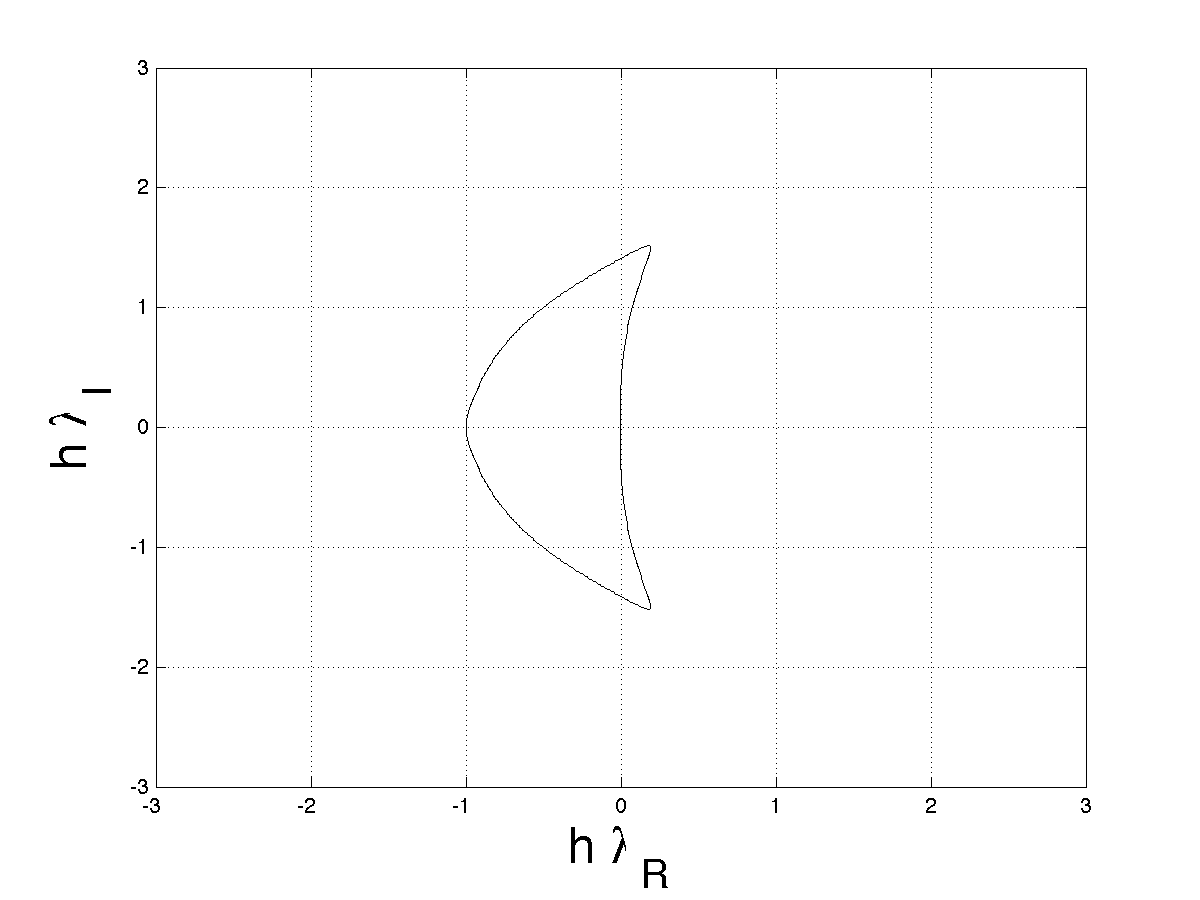
\includegraphics[width=0.8\textwidth]{andy_hw04_prb08_02.png}
  \caption{The stability region of a P-C method with Leap-Frog predictor and trapezoidal corrector.}
\end{figure}

\end{enumerate}

\clearpage
\newpage
{\huge \textbf{Appendix: Function code}}
\lstinputlisting[language=Matlab]{named_methods/andy_ME.m}

\noindent\rule{4cm}{0.4pt}
\lstinputlisting[language=Matlab]{named_methods/andy_IE.m}

\noindent\rule{4cm}{0.4pt}
\lstinputlisting[language=Matlab]{named_methods/andy_cRK.m}

\noindent\rule{4cm}{0.4pt}
\lstinputlisting[language=Matlab]{named_methods/andy_SE.m}

%% \lstinputlnsting[language=Matlab]{}

\end{document}
